
\chapter{Explicación de la aplicación}

En este capítulo se explicara como funciona la aplicación WEB diseñada para recoger y mostrar los datos de cada uno de los sensores.

\begin{figure}[!h]
	\centering
	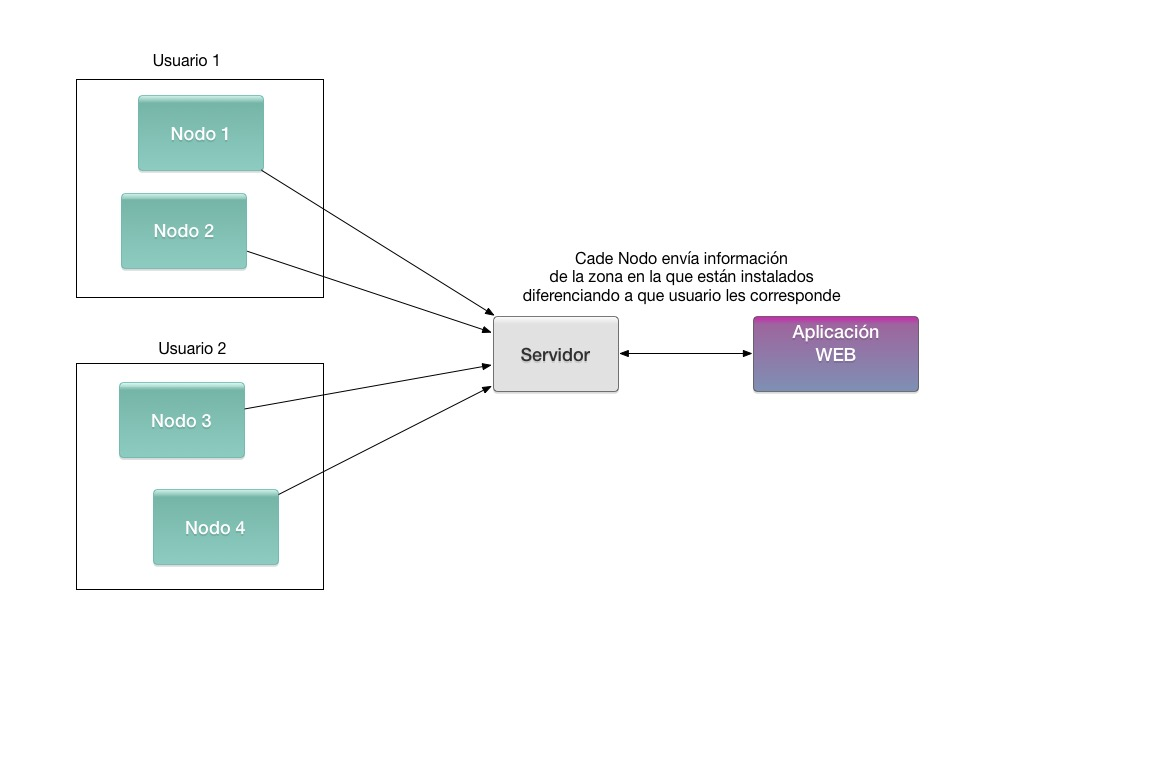
\includegraphics[width=0.9\linewidth]{figuras/montaje2}
	\caption{Esquema del funcionamiento de la aplicación}
	\label{fig:montaje2}
\end{figure}

\setlength{\parindent}{5ex}En la \textbf{Figura \ref{fig:montaje2}} se muestra el diagrama de la aplicación en el servidor en el que se dispone de una aplicación que recoge la información y la gestiona para que cada dispositivo o nodo se le pueda asignar a un usuario, este puede tener uno o muchos nodos y estos están recogiendo información independiente unos de otros y la almacena en la base de datos de manera organizada.
En la aplicación pueden haber muchos usuarios y cada uno puede almacenar la información de cada uno de sus nodos.

\clearpage

\section{Gestión de la información}

La gestión de la información es sencilla, se trata de una base de datos simple en la que se almacenará la información de los nodos, la estructura de esta base de datos esta creada automáticamente por Laravel la cual hay que especificarle el siguiente diagrama E-R:
\setlength{\parindent}{0ex}
\begin{figure}[!h]
	\centering
	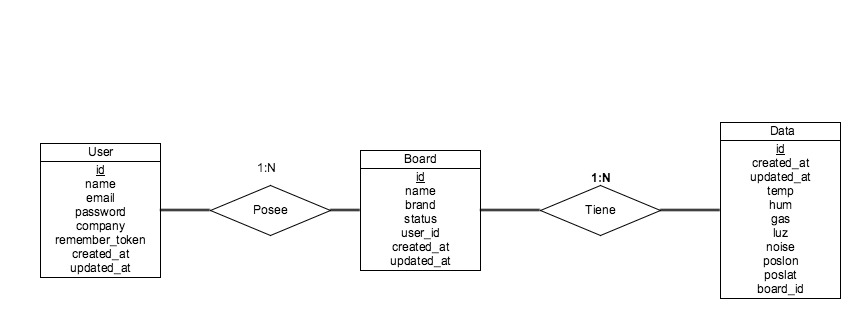
\includegraphics[width=0.9\linewidth]{figuras/diagramaer}
	\caption{Diagrama Entidad-Relación de la base de datos}
	\label{fig:bd1}
\end{figure}

Esta base de datos ha sido creada automáticamente por \textit{Artisan} de Laravel, la gestión automática crea la tabla de \textit{usuarios} y algunos campos por defecto como \textit{created\_at} y \textit{updated\_at} sin embargo el resto de los campos hay que añadirlos manualmente así como especificar los tipos de relación entre los campos, este es el código del fichero alojado en l\textit{aravel-tfg/database/migrations/tfgDatabase.php} que especifica estos campos en la BD.\\

\begin{lstlisting}[caption=Migración de la base de datos, label=migration]
class TfgDatabase extends Migration{
	/**
	* Run the migrations.
	* @return void
	*/
	public function up(){
		Schema::create('board', function (Blueprint $table) {
			$table->increments('id');
			$table->string('name');
			$table->string('brand');
			$table->string('status');
			$table->integer('user_id')->unsigned();
			$table->timestamps();
			$table->foreign('user_id')->references('id')->on('users');
		});
		Schema::create('data', function (Blueprint $table) {
			$table->increments('id');
			$table->timestamps();
			$table->string('temp');
			$table->string('hum');
			$table->string('gas');
			$table->string('luz');
			$table->string('noise');
			$table->string('poslon');
			$table->string('poslat');
			$table->integer('board_id')->unsigned();
			$table->foreign('board_id')->references('id')->on('board');
		});
	}
	/**
	* Reverse the migrations
	* @return void
	*/
	public function down(){
		Schema::drop('data');
		Schema::drop('board');
	}
\end{lstlisting}

Si se quisieran añadir mas sensores a la aplicación se tiene que insertar  una nueva entrada en la tabla data y luego aplicar la migración como se ha visto en el  \textbf{Código \ref{phpmigrate}}.

\section{Gestión del \textit{NodeTracker}}


\setlength{\parindent}{5ex}Una vez explicado como se almacena la información se procederá como puede acceder un usuario a la aplicación la cual se ha llamado \textit{NodeTracker}, Para ello hay que o bien instalarla y configurar los nodos a la dirección del servidor o bien acceder al servidor ya instalado en la siguiente URL:
\setlength{\parindent}{0ex}
\\
\url{http://84.123.151.120:8888/}

Una vez aparecerá el Login del Nodetracker, en el cual se podrá crear un usuario o entrar con uno ya disponible:

\begin{figure}[!h]
	\centering
	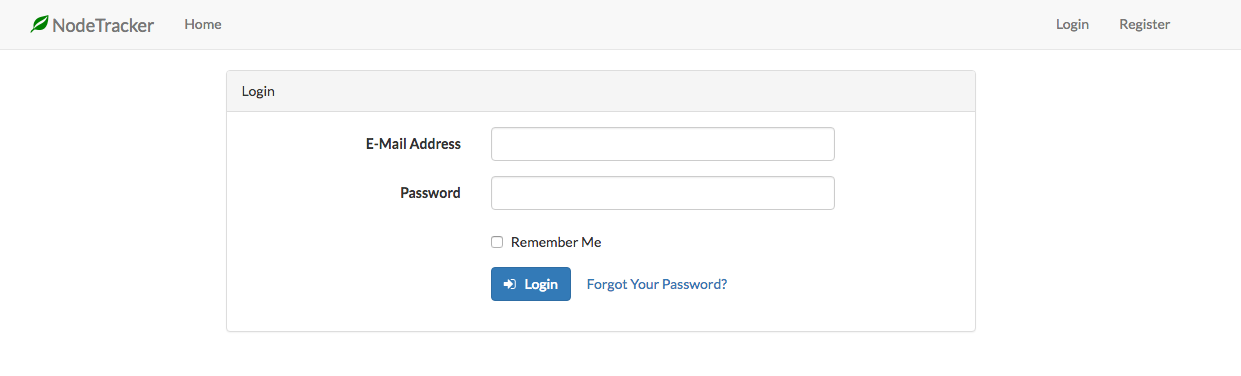
\includegraphics[width=1.0\linewidth]{figuras/loginnode}
	\caption{Login del NodeTracker}
	\label{fig:loginnode}
\end{figure}

Una vez Logueado en la aplicación se muestra lo que se ha denominado como el Home, un panel para la gestión de los diferentes nodos la cual incorporara la funcionalidad de editar el usuario o añadir nuevos nodos.

\begin{figure}[!h]
	\centering
	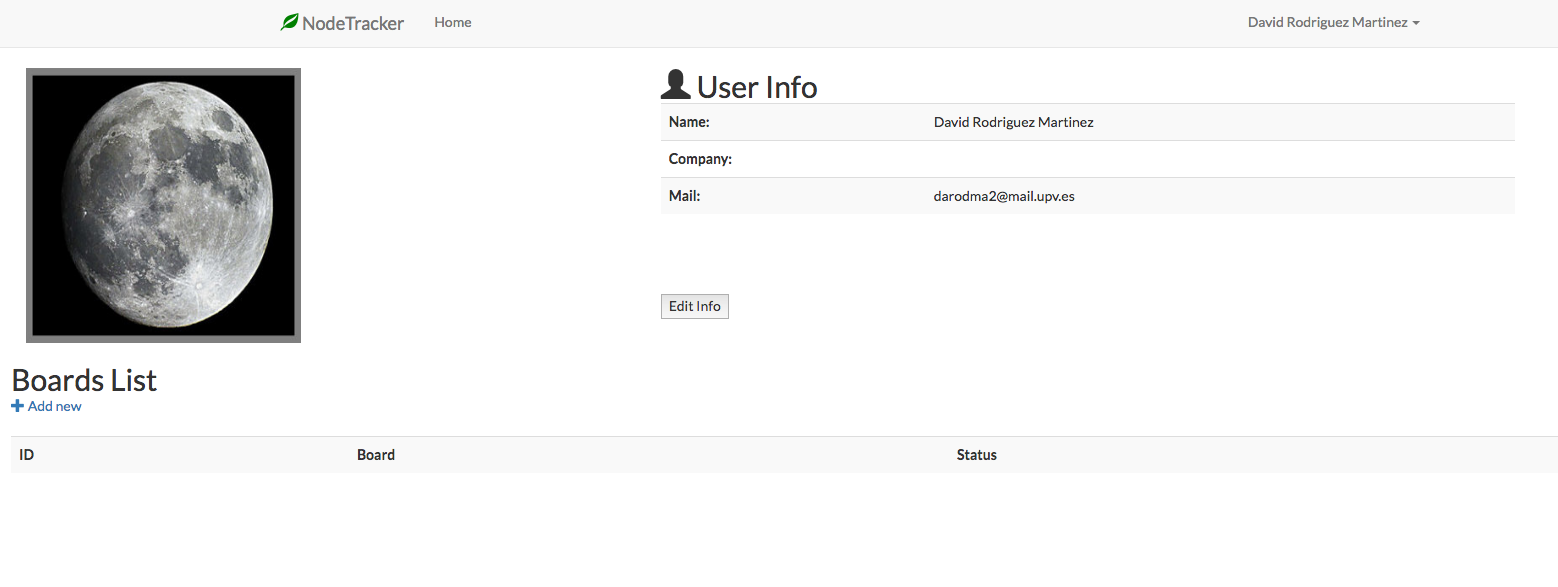
\includegraphics[width=1.0\linewidth]{figuras/homenode}
	\caption{Home del NodeTracker}
	\label{fig:homenode}
\end{figure}

Con un pequeño formulario se puede editar la información básica del usuario (\textbf{Figura \ref{fig:editusernode}}) y ademas como se había diseñado para esta aplicación se pueden añadir uno o mas nodos (\textbf{Figura \ref{fig:addnode}}), esta funcionalidad devolverá una ID en la tabla la cual se tendrá que modificar en el código del Arduino con el fin de que guarde la información correcta correspondiente al nuevo nodo en la base de datos. 

\begin{figure}[!h]
	\centering
	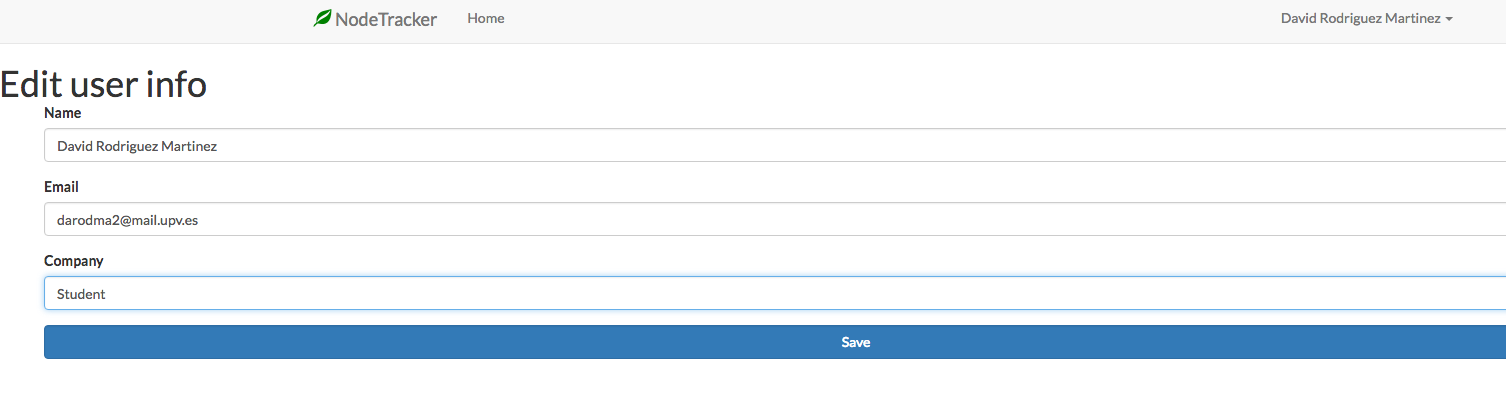
\includegraphics[width=0.7\linewidth]{figuras/edituser}
	\caption{Formulario de edición de usuarios del \textit{NodeTracker}.}
	\label{fig:editusernode}
\end{figure}

\begin{figure}[!h]
	\centering
	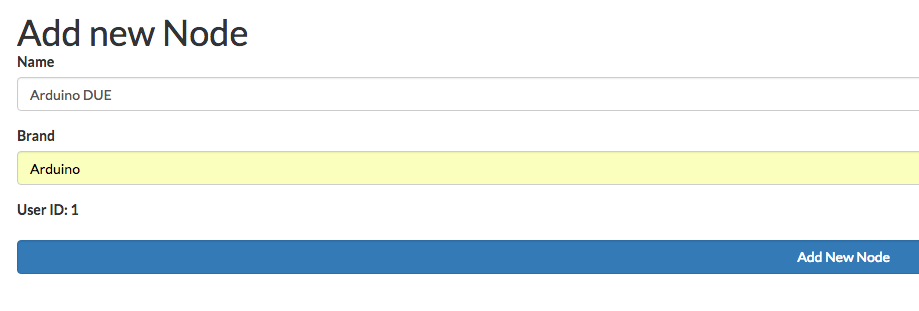
\includegraphics[width=0.7\linewidth]{figuras/addnode}
	\caption{Formulario para añadir un nuevo nodo al sistema.}
	\label{fig:addnode}
\end{figure}

Una vez creado para poder asignarlo al Arduino devolverá una ID para poder asignársela al nodo.

\begin{figure}[!h]
	\centering
	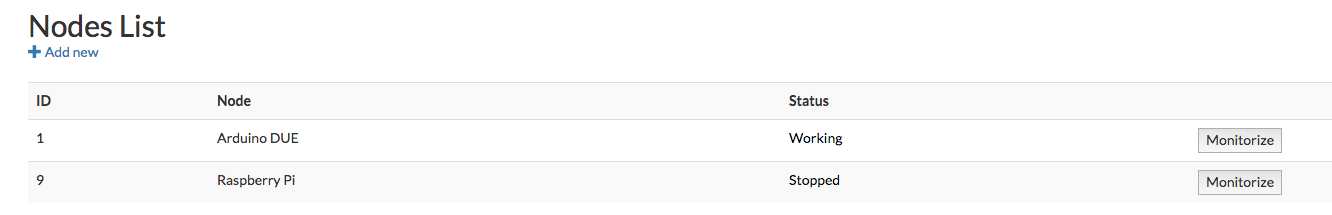
\includegraphics[width=1.0\linewidth]{figuras/nodelist}
	\caption{Lista de nodos disponibles}
	\label{fig:nodelist}
\end{figure}

En la \textbf{Figura \ref{fig:nodelist}} se puede ver la ID el nombre asignado y el estado del nodo que por defecto viene parado, para poder enlazar los nodos con la aplicación hay que visualizar la ID i añadirla en la función del código que recoge la ID en el Arduino, pero básicamente hay que cambiar en la String a enviar al servidor, por ejemplo si se quisiera enviar información desde una Raspberry Pi la cual la ID es 9, habrá que configurar la String tal que así:

\begin{lstlisting}[caption=Ejemplo para una ID diferente, label=getstringexaple]
192.168.1.16:8888/call?board_id= 8....
\end{lstlisting}

También esta el botón que redirigirá a la pagina de los reportes para poder visualizar la información obtenida que es la parte fuerte de la aplicación, es un panel donde se podrá visualizar la información o generar un reporte con la información recogida.
\clearpage

\section{Visualización  de la información}

\begin{figure}[!h]
	\centering
	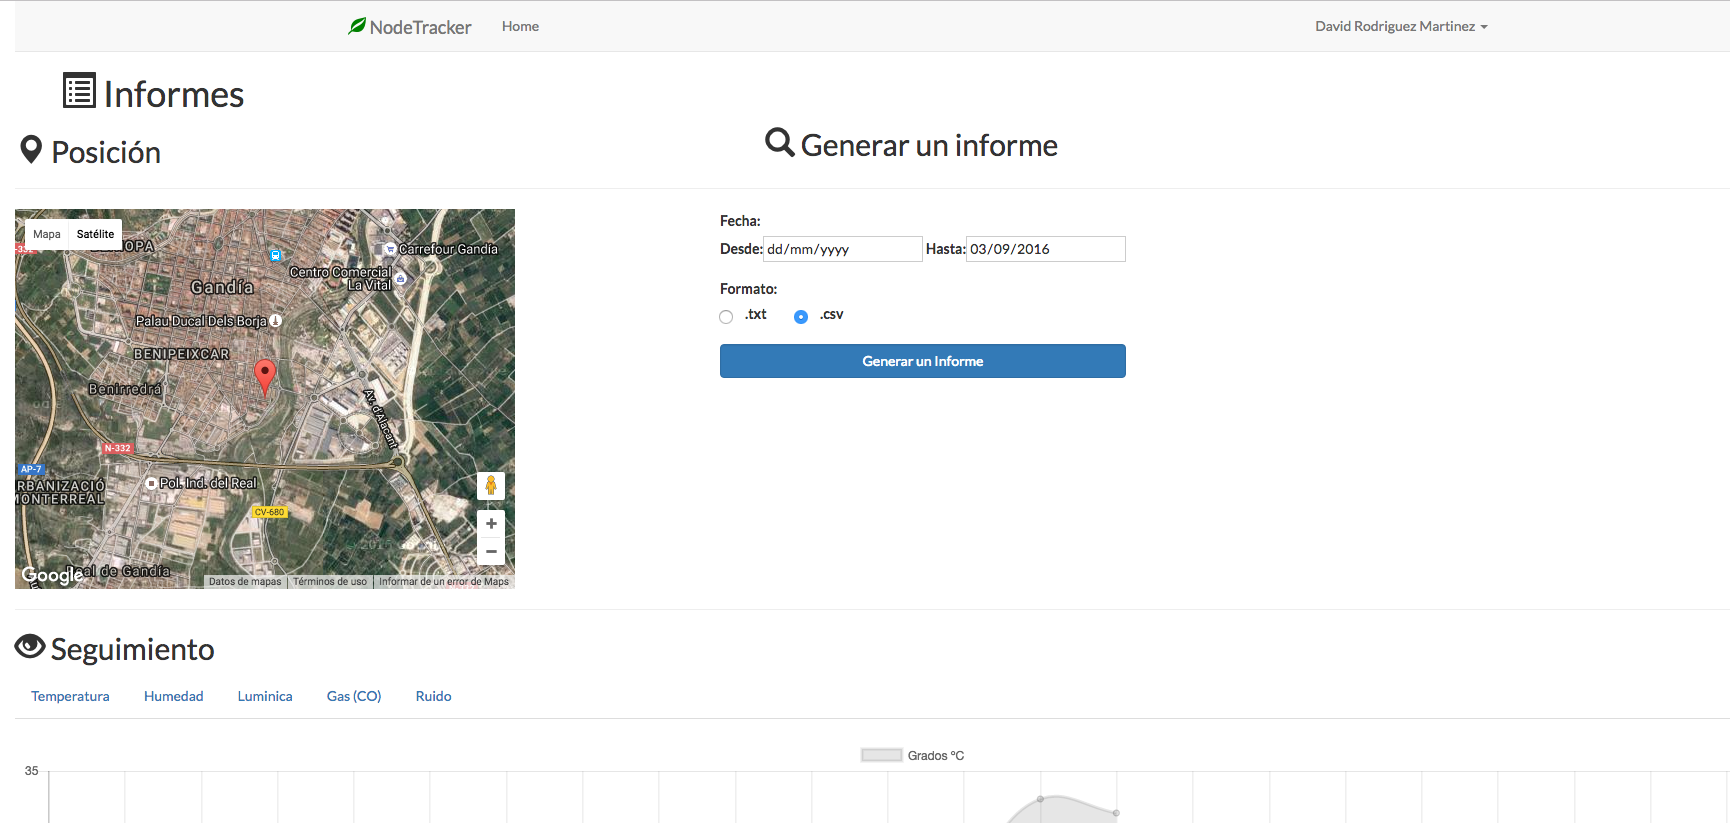
\includegraphics[width=1.0\linewidth]{figuras/nodereport}
	\caption{Pagina de monitorización de la aplicación}
	\label{fig:nodereport}
\end{figure}

Esta es la página en la que se podrá visualizar la informacion, consta de 3 secciones, un mapa para mostrar la ubicación de la última entrada a la base de datos, otra sección que se encargara de generar los reportes para poder trabajar con ellos, y una gráfica que intentara mostrar un progreso de la informacion recogida a lo largo del día.

\subsection{Posicionamiento}

Para ello esta el Mapa en la sección de \textit{Position} que gracias a la API de Google MAPS se ha podido implementar esta funcionalidad, en este caso el mapa es en vista satélite ya que al ser una aplicación medioambiental, se necesitara saber si el nodo esta en un núcleo urbano o en territorio natural, y aproximadamente a que altura se puede encontrar, costa o altas montañas. \textit{Para el ejemplo de la \textbf{Figura \ref{fig:mapimg}} se dispone de las coordenadas -0.180812 y 38.960541 que corresponden al termino municipal de Gandía.} 

\begin{figure}[!h]
	\centering
	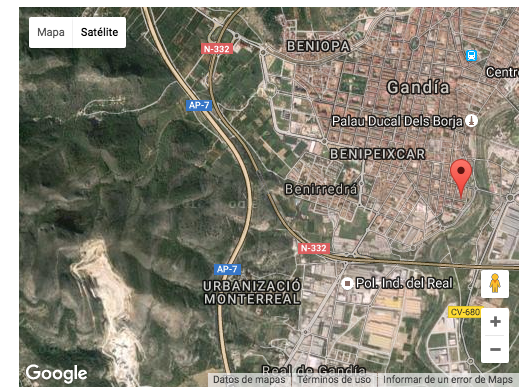
\includegraphics[width=0.5\linewidth]{figuras/mapimg}
	\caption{Mapa de la posición del nodo.}
	\label{fig:mapimg}
\end{figure}

\clearpage
Se ha implementado este mapa ( \textit{indicando en las opciones del mapa que su configuración de vista sea por satélite }) pues se puede apreciar cuando se trata de un núcleo urbano, terreno montañoso, ríos o mares con el fin de que cuando se recojan los datos el usuario tenga cierta informacion del área que se esta monitorizando, en el caso de la \textbf{Figura \ref{fig:mapimg}} se puede apreciar la montaña en la parte izquierda y el núcleo urbano en la parte derecha.



\subsection{Obtener un informe}

Se ha implementado una función para generar informes, llamada \textit{Reports} la cual generará un informe definido por un rango de fechas.

\begin{figure}[!h]
	\centering
	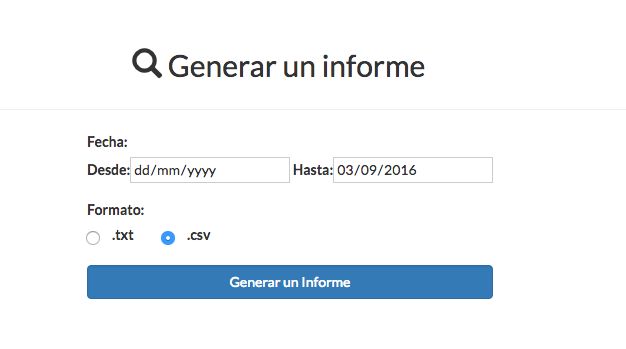
\includegraphics[width=0.8\linewidth]{figuras/nodereports2}
	\caption{Generación de Informes}
	\label{fig:nodereport}
\end{figure}

Esta función generara un informe en formato JSON de la informacion recogida cada minuto por el nodo unido a la aplicación, el resultado puede variar en el formato escogido en este caso .txt (texto plano) o .csv (Hojas de calculo para LibreOfice) para poder trabajarlas en otras aplicaciones o realizar migraciones de estas, muy útil para la minería de datos que, utilizando programas en R o Python se puede trabajar este formato JSON.

\subsection{Seguimiento de la información}

Por ultimo el la función de monitorización, llamada \textit{seguimiento} se ha implementado una gráfica utilizando la API de Chart.js que permitirá realizar un seguimiento los valores recogidos en cada hora de ese mismo día realizando un promedio de los valores obtenidos en esa hora del día, ya que implementar cada minuto seria visualmente cargado y podría desestabilizar la gráfica si se presentan valores anómalos. 
Ademas presenta una gráfica diferente para cada valor a medir (temperatura, humedad, gases, luz y ruido) que implementado con AJAX realiza el cambio de gráficos sin necesidad de refrescar la página.

Este es el código que permite cambiar de gráfico sin necesidad de cambiar toda la pagina\cite{ajax}:\\

\begin{lstlisting}[caption=Selector de Graficos, label=graficsel]
 <script>
	    function cambiarPestanna(divc,divc) {
	    divc = document.getElementById(divc.id);
	    listaPestannas = document.getElementById(divc.id);
	    cdivc = document.getElementById('c'+divc.id);
	    listacPestannas = document.getElementById('contenido'+divc.id);
	    i=0;
		while (typeof listacPestannas.getElementsByTagName('div')[i] != 'undefined'){
		    $(document).ready(function(){
			    $(listacPestannas.getElementsByTagName('div')[i]).css('display','none');
			    $(listaPestannas.getElementsByTagName('li')[i]).css('background','');
			    $(listaPestannas.getElementsByTagName('li')[i]).css('padding-bottom','');
		    });
		    i+=1;
	    }
	    $(document).ready(function(){
		    $(cdivc).css('display','');
		    $(divc).css('padding-bottom','2px');
	    });
    }
</script>
\end{lstlisting}

Esta función recoge todas las ventanas que coinciden con el identificador pues cuando se seleccione el enlace recogerá a cual va cambiar, luego recorre todos los disponibles y los oculta para mostrar la gráfica asignada a la pestaña.

Estas son dos ejemplos de las gráficas para mostrar la informacion recogidas por el nodo:

\begin{figure}[!h]
	\centering
	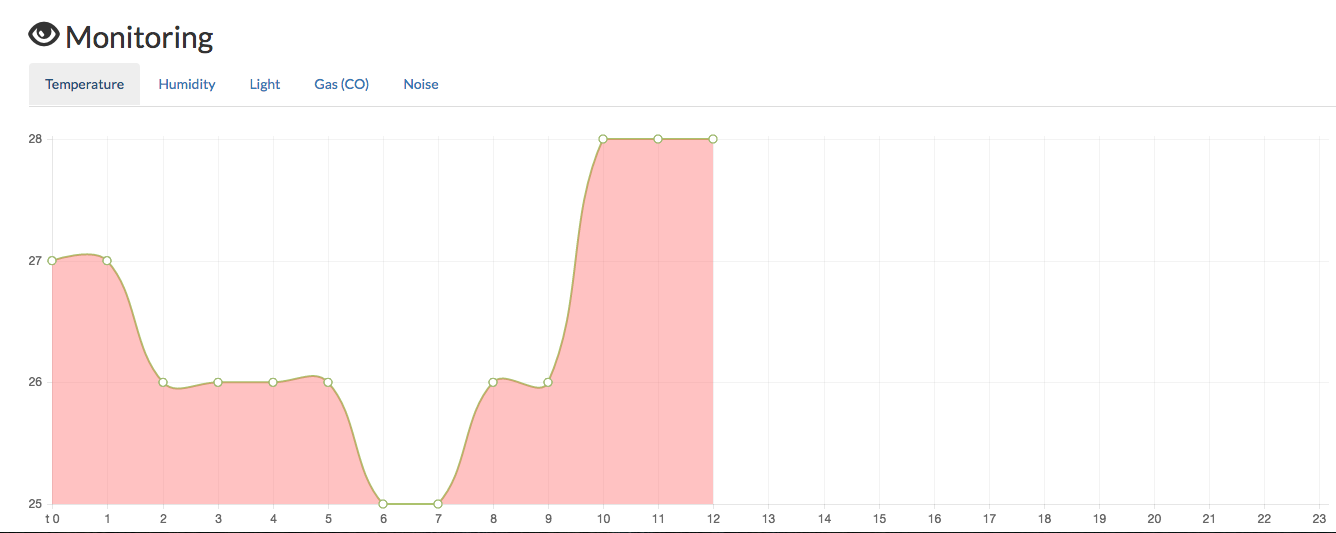
\includegraphics[width=0.9\linewidth]{figuras/nodereports3}
	\caption{Gráfica perteneciente a la temperatura en el seguimiento}
	\label{fig:nodereport}
\end{figure}

\begin{figure}[!h]
	\centering
	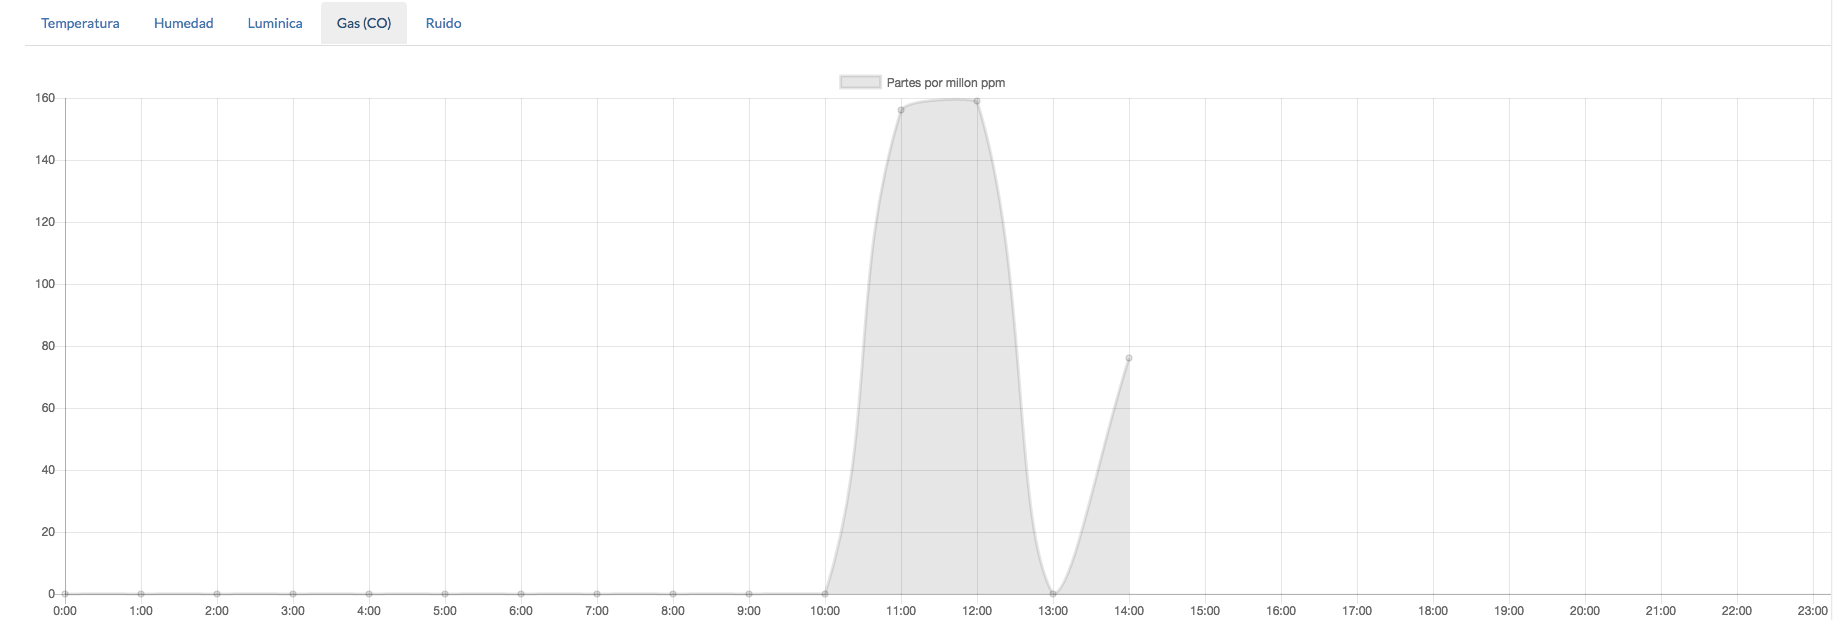
\includegraphics[width=0.9\linewidth]{figuras/node4}
	\caption{Gráfica perteneciente a la contaminación por CO en el seguimiento}
	\label{fig:nodereport}
\end{figure}

(Uno de los principales problemas que se ha tenido a la hora de diseñar esta gráfica era que cuando recibía los datos esta no interpretaba bien la hora así que al dibujar el gráfico empezaba pero se ha solucionado aplicando un 0 a cada hora que el nodo ha estado deshabilitado con el fin de prevenir errores en las lecturas de la aplicación.

También comentar que debido a los numerosos cambios de formato de una versión a otra de Chart.js la informacion es muy confusa pues en cada versión cambia la forma de implementar los atributos de la gráfica y por eso ha resultado muy complicado añadir una magnitud a los valores del eje Y por lo que se ha tenido que implementar con una leyenda que informe al usuario de la magnitud que se esta empleando para medir en esa gráfica.

Otro problema es la selección del color, en este caso queda con color gris aunque se le esta asignando un color y puede ser debido a lo descrito anteriormente y pueda ser una llamada errónea en la librería)

Aquí se presenta un ejemplo de una gráfica en las primeras de la librería de Chart.js:

\begin{figure}[!h]
	\centering
	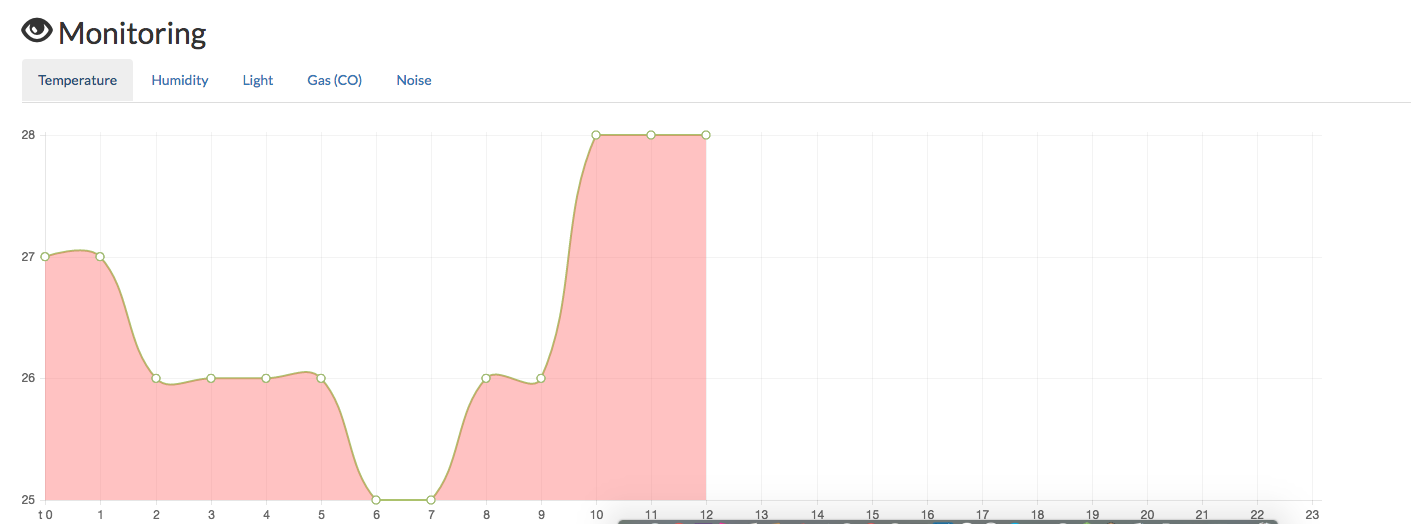
\includegraphics[width=0.7\linewidth]{figuras/charjs}
	\caption{Gráfica perteneciente a la Temperatura (\textit{versión antigua Chart.js)}}
	\label{fig:nodereport}
\end{figure}



